\section{Interface}
\label{sec:interface-ssa}

While the core code-base has been designed and implemented
  to be easily accessible to those who wish to use it directly or extend it,
  the expected everyday interface to this project is
  the graphical tool presented below.
It fully supports the creation and documentation of
  self-stabilizing algorithms,
  rules,
  predicates,
  and moves
  using a combination of textual and graphical interfaces.
Since the bundle format is self-contained,
  all of these objects \Dash
  predicates, moves, and algorithms \Dash
  can be saved and distributed to colleagues
  that are using the same or derivative software.

\subsection{Predicates and Moves}
As reflected in the logical representation
  (see~\autoref{sec:logic-repr:self-stab-algor}),
  self-stabilizing algorithms persist as a collection
  of predicates and moves.
As such, this tool supports the convenient creation of these basic components.

Predicates and moves can be created using the graphical interface,
  but it should be noted that the \emph{definition} of these is left
  as plain-text input.
(See also~\autoref{task:gui-syntax-highlighting} and~\autoref{task:gui-definition-wrapping}.)
(This definition will be written verbatim to disk;
  see \autoref{sec:logic-repr:predicate-move}.)
To create them, navigate to the \menu{Predicates} or \menu{Moves} tabs
  and click the "add" button beneath the list on the far left
  (\autoref{fig:ex:predicates}).
This will add an empty item \Dash in this case, a predicate \Dash to the list.
Editing its \menu{Predicate > Name} field will update its name in the list accordingly.
Fill in the \menu{Predicate > Author}, \menu{Predicate > Date},
  and \menu{Predicate > \TeX} fields as appropriate.

\begin{warning}
  When giving any entity a name, be sure to edit it character-by-character starting from the end,
    deleting using \emph{only} the backspace \keys{\backspace} key.
  No other behavior has been tested, but consistent crashes occur when attempting to delete multiple
    characters via a selection.
  See~\autoref{task:update-name}.
\end{warning}

When you are ready to provide a definition,
  simply enter it in the large text area beneath the
  \menu{Predicate > File} and \menu{Predicate > Description} fields.
The definition must be in Python~3 syntax~\autocite{python3:ref}.
\begin{warning}
  Due to the imperfect implementation of the interface,
    the last line of the definition string is \emph{always} lost.
  Unless you terminate the definition with a newline character,
    the last line you give will be lost.
  For example, if the definition is only one line (say "return n['marked']"),
    this entire definition will be lost.
  This is a bug noted as part of~\autoref{task:definition-newline}.
\end{warning}

\begin{warning}
  When you have finished editing the definition for a predicate or move,
    the file is immediately written to disk.
  This action cannot be undone and is unaffected by the \menu{File Manager > Save Bundle} operation.
  This can be mitigated by~\autoref{task:temp-files}.
\end{warning}

\subsection{Documentation}
All entities \Dash predicates, moves, rules, and algorithms \Dash support documentation in various manifestations.
In the graphical interface, these fields include the author,
  a name,\footnote{Required and must be unique.  See~\autoref{sec:bundle-descr-docum}.}
  a description, and \TeX nical documentation.
\paragraph{\TeX nical documentation}
When exporting an algorithm as a PDF (processed via \TeX\slash\TikZ),\footnote{%
  Not yet supported via the graphical interface.
  See~\autoref{task:texport}.}
  the \TeX nical documentation for each entity is given special treatment.
As bundles should be self-sufficient,
  there is an easy syntax to use to denote the properties of a node.
Considering \Algorithm{IndSet}, the quality of being \enquote*{in the set}
  may be denoted as \texttt{\QuoteLiteral{marked}(n) = 1}.
Note the literal double quotes (the single character \texttt{\char`"}) around the function name;
  in addition to clearly describing the purpose of a value,
  this notation will be replaced as appropriate by
  the more verbose (but correct) "\operatorname{marked}".

It should be noted that {\TeX} export is not yet functional in the core tool;
  this syntax is merely set in place to guide further development.
\todo{Update as necessary}
See~\autoref{task:texport}.
\subsection{Algorithms}

Algorithm assembly is fully supported using the graphical interface.
To create an algorithm, simply click the \menu{Algorithm > add} button
  underneath the list of algorithms to the right.
(This list will be empty in a new bundle.)
Once this has been done, giving the Algorithm a name (via the \menu{Algorithm > Name} field)
  will update its text in the listing accordingly.

The process is similar to add new rules to the algorithm.
To create a new rule, simply press the \menu{Algorithm > Rules > add} button under the list of rules.
Give it a predicate via the drop-down (which is populated by the list of predicates in their tab)
  and transfer moves between the master list on the left (similarly populated) and the rule's list on the right
  using the angle bracket buttons (\menu{{>}} and \menu{{<}}) between them.

\subsubsection{Special Instructions}

Unfortunately, this tab is especially buggy (see~\autoref{task:alg-aggr}).
Special care must be taken to ensure that the interface does not crash.
For reference, consider the following script when creating these entities.
This script creates the algorithm \Algorithm{IndSet} as part of a new bundle.

\begin{enumerate}
\newcommand\bash[1]{\texttt{#1}}%{\fcolorbox{gray}{green!15}{{\ttfamily\footnotesize #1}}}
\item Open the interface from the terminal: \bash{python3 gui.py}
\item Navigate to the \menu{Algorithms} tab by clicking on it.
\item Create a predicate to test if a node should mark.
  \begin{enumerate}
  \item Navigate to the \menu{Predicates} tab.
  \item Click \menu{Predicates > add} to create a new predicate.
    Select the predicate when it appears in the list box.
  \item Click \menu{Predicates > Name} and, using either the arrow keys or the mouse, navigate to the end.
    Be careful not to select any text; this has not been tested (and in some cases, causes an exception).
    See~\autoref{task:update-name}.
  \item Pressing backspace \keys{\backspace} to delete the existing text,
    rename the predicate to \enquote{node should mark}.
  \item Give the entity additional metadata through the
    \menu{Predicates > Author},
    \menu{Predicates > Date},
    \menu{Predicates > \TeX},
    \menu{Predicates > Description}, and
    \menu{Predicates > File Name} fields.
  \item Provide the definition provided in~\autoref{lst:ex:should-mark},
    taking care to add the terminal newline (see~\autoref{task:definition-newline}).
  \end{enumerate}
\item Create a predicate to test if a node should unmark.  Repeat the
  above for a predicate named \enquote{node should unmark}, with the
  definition provided in~\autoref{lst:ex:should-unmark}.
\item Select the previous predicate to save the current one.
  (See~\autoref{task:temp-files}.)
  After this, the interface should look similar to~\autoref{fig:ex:predicates}.
\item Create a rule to mark a node.
  Repeat the process for a move (under the \menu{Moves} tab)
    named \enquote{mark node} with the definition given in~\autoref{lst:ex:mark}.
\item Create a rule to unmark a node.
  Repeat the process for a move
    named \enquote{unmark node} with the definition given in~\autoref{lst:ex:unmark}.
\item Select the previous move to save the current one.
  (See~\autoref{task:temp-files}.)
\item Create an algorithm entity called \enquote{Independent Set}.
\begin{enumerate}
\item Click \menu{Algorithms > add} to create an algorithm entity.
\item Edit \menu{Algorithms > Name} using the same procedure as before.
  Call the algorithm \enquote{Independent Set}.
\item Repeat this process for \menu{Algorithms > Author} and \menu{Algorithms > Date},
  being careful to give \menu{Algorithms > Date} in the correct format~(see~\autoref{task:dates}).
\end{enumerate}
\item Add a rule to mark a node.
  \begin{enumerate}
  \item Click \menu{Algorithms > Rules > add} to create a new rule.
  \item Repeat the process above to give the rule the name
    \enquote{ENTER}, taking care to edit the correct field
    (\menu{Algorithms > Rules > Name}).
  \item Edit \menu{Algorithms > Rules > Author} as appropriate.
  \item Edit \menu{Algorithms > Rules > Predicate} to \enquote{node
      should mark}.  When the name given matches the name of an
    existing predicate, it will turn color from red to black.
  \item In the listbox on the left, select \enquote{mark node} and
    click \menu{Algorithms > Rules > {>}}.
  \end{enumerate}
\item Add a rule to unmark a node.  Repeat the above for a rule named
  \enquote{LEAVE} with the predicate \enquote{node should unmark} and
  the single move \enquote{unmark node}.
\item Select the previous rule to save the current one.
  After this, the interface should look similar to~\autoref{fig:ex:algorithm}.
\item Navigate to \menu{File Manager}.
\item Give the a full path of the file you wish to write
  (or a path relative to the working directory the interface was started from)
  in \menu{File Manager > Path}.
\item Click \menu{File Manager > Save Bundle}.
\item Close the interface.
  The bundle now exists at the path specified in \menu{File Manager > Path}.
\end{enumerate}

\begin{figure}[p]
  \centering
  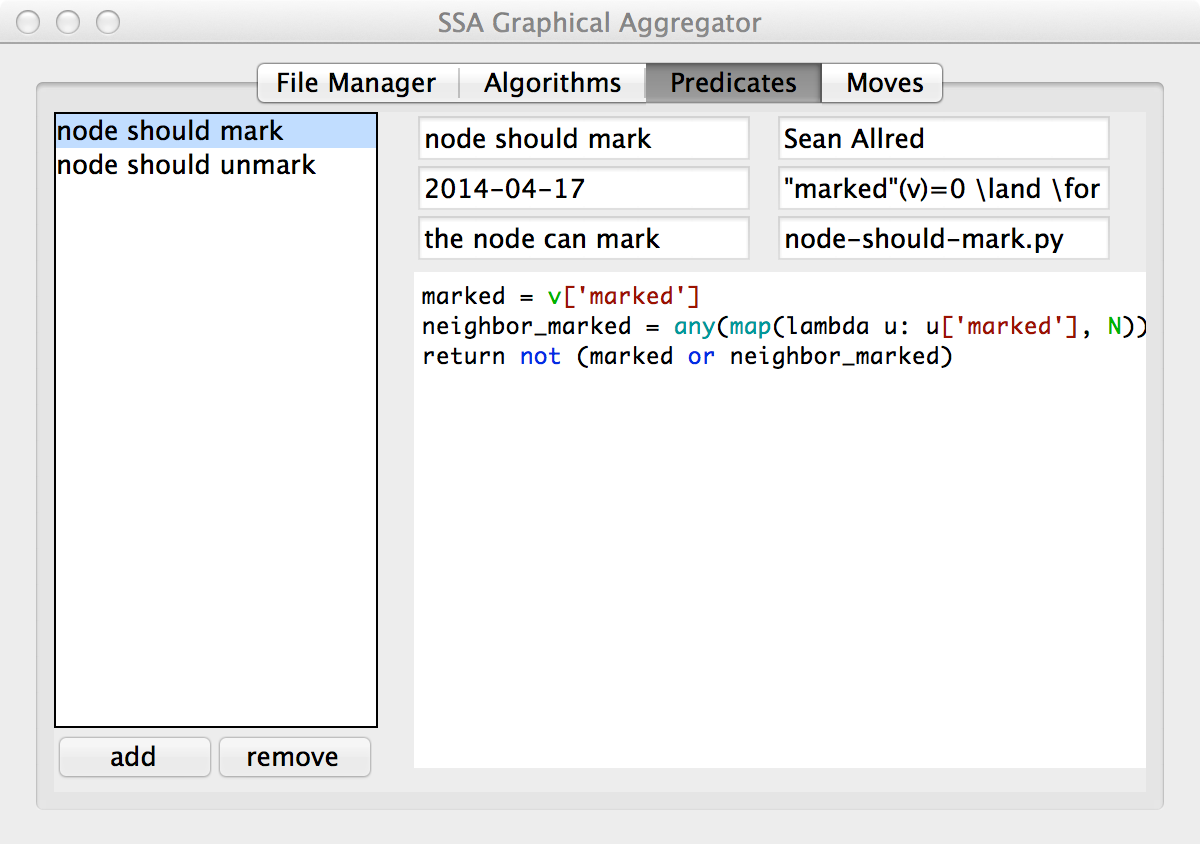
\includegraphics[height=.4\textheight]{figs/2}
  \caption{The interface looking at a completed predicate.}
  \label{fig:ex:predicates}
\end{figure}
\begin{figure}[p]
  \centering
  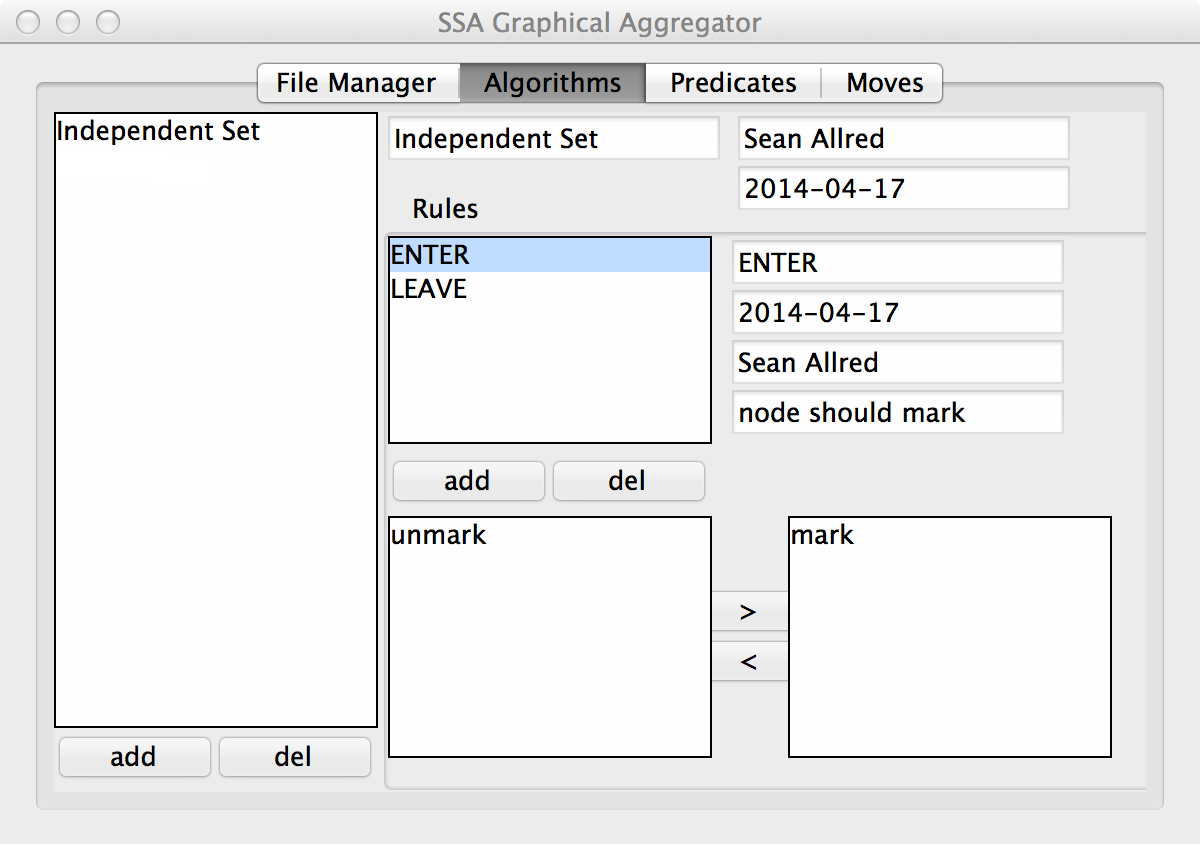
\includegraphics[height=.4\textheight]{figs/4}
  \caption{The interface looking at a completed algorithm.}
  \label{fig:ex:algorithm}
\end{figure}

\begin{warning}
  When \enquote*{overwriting} a bundle, the operation is union-with-overwrite.
  This means that the tool will not overwrite files that do not exist in the bundle it wishes to write,
    but it will overwrite those it has a record for.
  This means that the bundle description document \emph{will} be overwritten,
    but perhaps other files that existed previously will remain.
  If this is a possibility, it is a good idea to load the bundle first so that different names can be given to entities.
\end{warning}

\subsection{Creating, Loading, and Saving Bundles}
\label{sec:iface:saving}

To save and load bundles, navigate to \menu{File Manager} tab.
Enter the \emph{full}, \emph{absolute} path of the bundle you wish to load and,
  taking special care not to press \menu{File Manager > Save Bundle}
  (as this will overwrite it),
  press \menu{File Manager > Load Bundle}.
Successively loading bundles will aggregate them under a union operation
  to allow for distributed work toward larger and larger bundles.

\begin{figure}
  \centering
  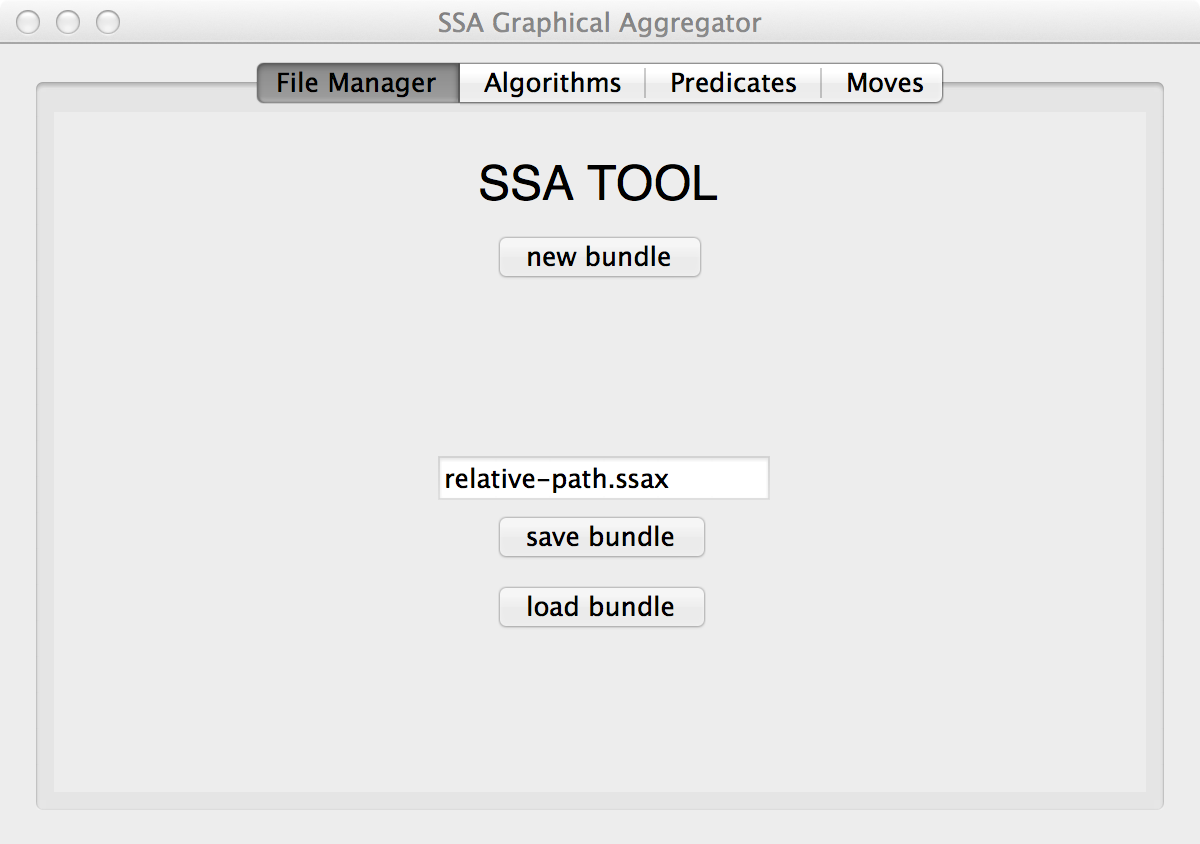
\includegraphics[width=\textwidth]{figs/3}
  \caption{The file management interface}
  \label{fig:iface:fmgr}
\end{figure}

%%% Local Variables: 
%%% mode: latex
%%% TeX-master: "../smp.tex"
%%% reftex-cite-format: "\\autocite{%l}" 
%%% TeX-PDF-mode: t 
%%% TeX-command-default: "arara"
%%% TeX-engine: xetex
%%% End: 
